\subsection{Wi-Fi}

The \glspl{cpe} analyzed use a very common technique to assign different \glspl{essid} to distinct \gls{cpe}s. The last 4 hexadecimal digits of the \gls{mac} address of one of its network interfaces are appended to a fixed prefix, generating a reasonably unique name for the \gls{wifi} networks. Devices that support the 5 \gls{G}\gls{Hz} band add a \texttt{-5G} suffix to the generated name and assign it to the \gls{essid} of the faster network, distinguishing it from the 2.4 \gls{G}\gls{Hz} network. \glspl{cpe} 4 and 5 also advertise the 5 \gls{G}\gls{Hz} network without the \texttt{-5G} suffix, with intent to upgrade compatible devices on the 2.4 \gls{G}\gls{Hz} band to the 5 \gls{G}\gls{Hz} band when appropriate.

Almost all \glspl{cpe} in the research use a common, but unsafe, derivation method for the \gls{wifi} passphrase by using part of the \gls{bssid} of the network. On \glspl{cpe} 2, the password is the last 10 hexadecimal digits of the \gls{bssid}. The password for \glspl{cpe} 0, 1, 4, and 6 is the substring from the third to the tenth hexadecimal digit of the \gls{bssid} appended by the last to characters of the 2.4 \gls{G}\gls{Hz} network \gls{essid}. \glspl{cpe} 0, 1, 2, and 4 use the uppercase version of the hexadecimal \gls{mac} address, while \gls{cpe} 6 uses the lowercase version.

\glspl{cpe} 3, 5, and 7 have passphrases that could not be identified to be derived from any other information of the equipment. But, by analyzing other \glspl{cpe} of the same model, it was confirmed that their values follow a pattern.

Given that none of the \glspl{cpe} are compatible with \gls{wpa}3, an offline brute-force attack can be performed. With the patterns found on passwords of \glspl{cpe} 3, 5, and 7, the attack may succeed in a reasonable time.

Additionally, \glspl{cpe} 0 to 4 are using \gls{wpa} as security protocol alongside \gls{wpa}2. Meaning that even with a strong passphrase, it is not possible to ensure that the network is safe. \glspl{cpe} 6 and 7 are susceptible to the same class of problems on their 2.4 \gls{G}\gls{Hz} network, \gls{wpa} is enabled on \gls{cpe} 7 and \gls{cpe} 6 strangely enables \gls{tkip} with \gls{wpa}2 even though \gls{wpa} support is disabled.

Table 9 presents the patterns found on the passphrase of each \gls{cpe}. It also indicates the maximum brute-force time needed to crack the password on a p3.2xlarge \gls{aws} \gls{ec2} Instance \cite{aws_ec2_p3_instances} given the benchmark presented in Figure \ref{figure:hashcat_benchmark_wpa_pmk}. The \glspl{cpe} with 0s brute-force time can have their password derived from other information in constant time.

\begin{table}[h]
    \makebox[\linewidth]{
        \begin{tabular}{c|c|c}
            \thead{\gls{cpe} Identifier} & \thead{Passphrase Pattern} & \thead{Brute-Force Time} \\
            \hline
            \gls{cpe}-0 & \texttt{upper(\gls{mac}{[}2:10{]} + \gls{essid}{[}-2:{]})} & 0s \\
            \gls{cpe}-1 & \texttt{upper(\gls{mac}{[}2:10{]} + \gls{essid}{[}-2:{]})} & 0s \\
            \gls{cpe}-2 & \texttt{upper(\gls{mac}{[}2:{]})} & 0s \\
            \gls{cpe}-3 & \texttt{{[}0-9A-Za-z{]}\{10\}} & 565871h \\
            \gls{cpe}-4 & \texttt{upper(\gls{mac}{[}2:10{]} + \gls{essid}{[}-2:{]})} & 0s \\
            \gls{cpe}-5 & \texttt{{[}0-9A-Za-z{]}\{10\}} & 565871h \\
            \gls{cpe}-6 & \texttt{lower(\gls{mac}{[}2:10{]} + \gls{essid}{[}-2:{]})} & 0s \\
            \gls{cpe}-7 & \texttt{{[}0-9A-F{]}\{10\}} & 45min \\
        \end{tabular}
    }
    \caption{Wireless Network Passphrase Pattern of the \gls{cpe}s}
    \label{table:cpes_wifi_pattern}
\end{table}

\begin{figure}[h]
    \centering
    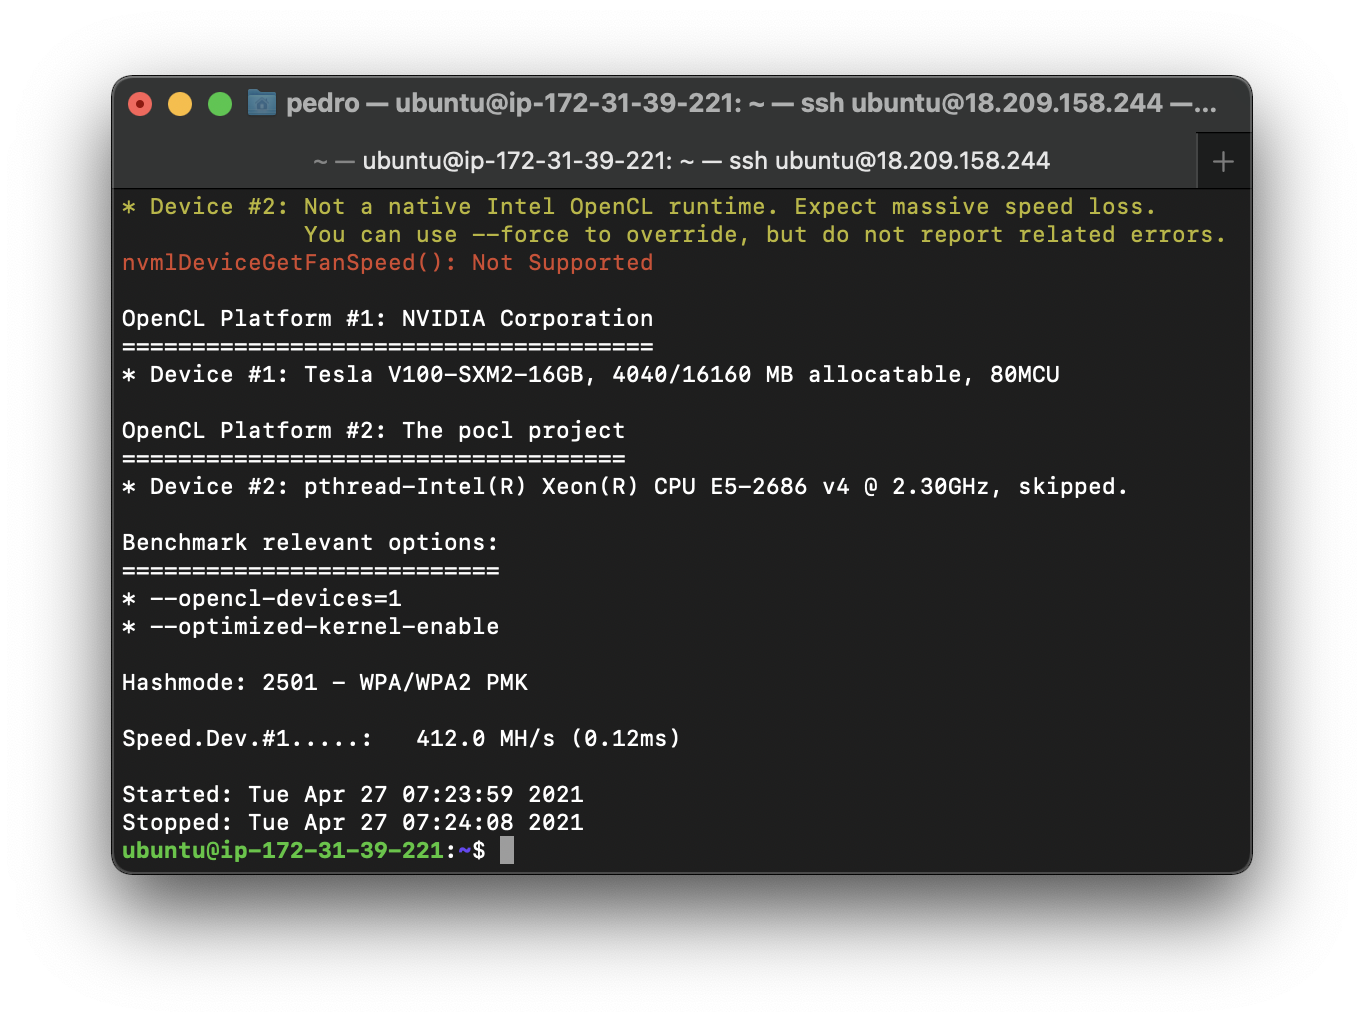
\includegraphics[width=\linewidth]{contents/configuration-analysis/wifi/hashcat-benchmark-wpa-pmk.png}
    \caption{Hashcat \gls{wpa} Benchmark on a p3.2xlarge \gls{aws} \gls{ec2} Instance}
    \label{figure:hashcat_benchmark_wpa_pmk}
\end{figure}

Additionally, all \glspl{cpe} have \gls{wps} enabled by default and allow authentication via \gls{pbc} and \glspl{cpe} 2 and 5 also can authenticate via \gls{pin}. The \glspl{cpe} were not found to be vulnerable to a \gls{wps} brute-force attack.

The \gls{pin} used on \gls{cpe} 2 is a random number that could not be recognized as a derivation of other information and was found in the backup partition of the \gls{eprom}, possibly indicating that it could have been assigned while in the factory. The \gls{pin} can be reset to a random value via the \gls{http} management interface and persists between reboots, but the original value is restored when the device is factory reset. After multiple resets, none of the generated \glspl{pin} do not seem to relate to previously generated \gls{pin}s, indicating that the \gls{prng} is not reset to a known state on factory restores.

On \gls{cpe} 5, there is no indication on its web interface that a \gls{wps} \gls{pin} can be used to authenticate to the network as well. Furthermore, the \gls{pin} is set to 12345670 by default and there is no procedure to regenerate the \gls{pin} or disable it via regular means. It was only possible to change \gls{wps} settings by exporting the configuration file, decrypting it, modifying the \gls{pin} value or disabling the authentication method, encrypting the modified file, and finally importing it back to the \gls{cpe}.

\FloatBarrier
